\documentclass{beamer}
\usepackage{latexsym}
\usepackage{graphicx}
\usepackage{listings}

\usetheme{Warsaw}

\title{Chapter 7}
\subtitle{Ensemble Classifiers}

\begin{document}
\maketitle

\begin{frame}
  \frametitle{Learning with ensembles}
  \begin{itemize}
  \item Our goal is to combined multiple classifiers
  \item Mixture of experts, e.g. 10 experts
  \item Predictions more accurate and robust
  \item Provide an intuition why this might work
  \item Simplest approach: majority voting
  \end{itemize}
\end{frame}

\begin{frame}
  \frametitle{Majority voting}
  \begin{itemize}
  \item Majority voting refers to binary setting
  \item Can easily generalize to multi-class: plurality voting
  \item Select class label that receives the most votes (mode)
  \end{itemize}
  \vspace{0.2in}
  \center
  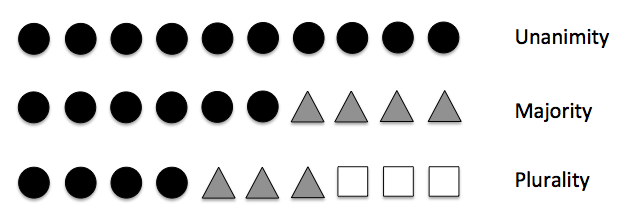
\includegraphics[scale=0.4]{Code/ch07/images/07_01.png}
\end{frame}

\begin{frame}
  \frametitle{Combining predictions: options}
  \begin{itemize}
  \item Train $m$ classifiers $C_1,\dots,C_m$
  \item Build ensemble using different classification algorithms (e.g. SVM, logistic regression, etc.)
  \item Use the same algorithm but fit different subsets of the training set (e.g. random forest)
  \end{itemize}
\end{frame}

\begin{frame}
  \frametitle{General approach}
  \center
  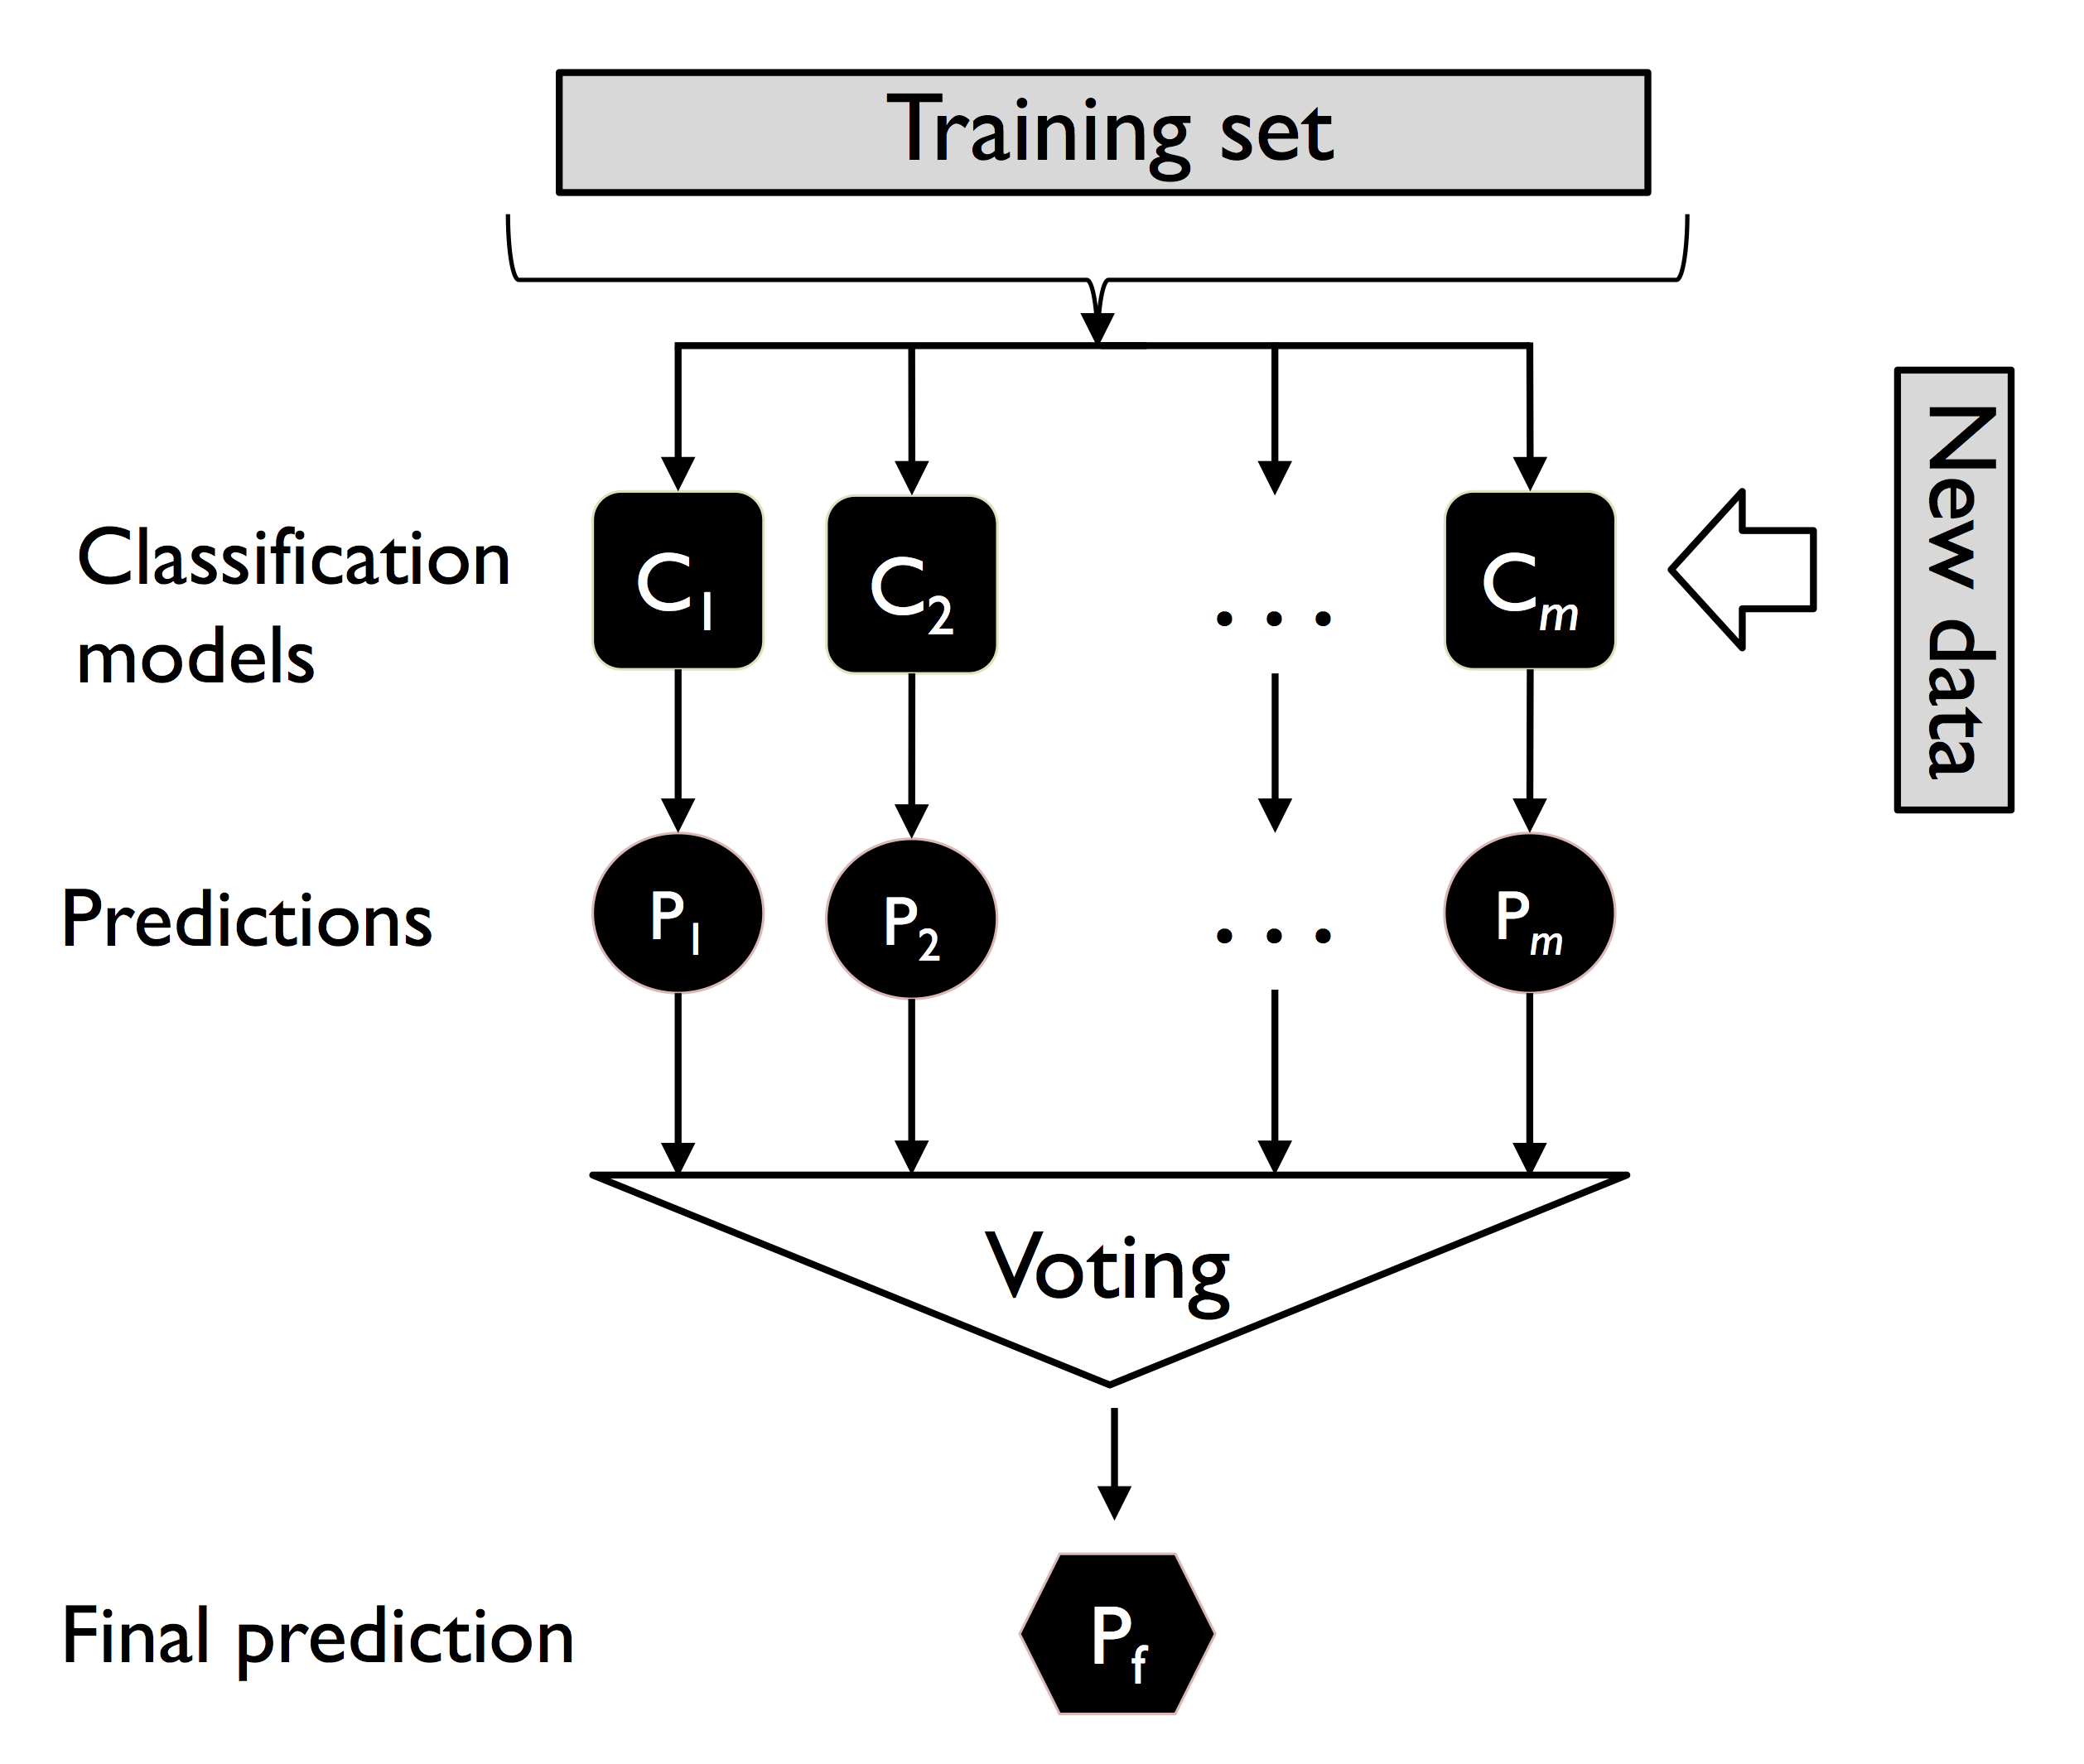
\includegraphics[scale=0.35]{Code/ch07/images/07_02.png}
\end{frame}

\begin{frame}
  \frametitle{Combining predictions via majority voting}
  We have predictions of individual classifiers $C_j$ and need to select the final class label $\hat{y}$
  \[
  \hat{y} = mode \{ C_1 (\mathbf{x}), C_2 (\mathbf{x}), \dots, C_m (\mathbf{x}) \}
  \]
  For example, in a binary classification task where $class_1 = -1$ and $class_2 = +1$, we can write the majority vote prediction as follows:
  \[
  C(\mathbf{x}) = sign \Bigg[ \sum_{j}^{m} C_j (\mathbf{x}) \Bigg] = \begin{cases}
        1 & \text{ if } \sum_j C_j (\mathbf{x}) \ge 0 \\
        -1 & \text{ otherwise }
     \end{cases}
  \]
\end{frame}

\begin{frame}
  \frametitle{Intuition why ensembles can work better}
  Assume that all $n$ base classifiers have the same error rate $\epsilon$. We can expresss the probability of an error of an ensemble can be expressed as a probability mass function of a binomial distribution:
  \[
  P(y \ge k) = \sum_{k}^{n} \binom{n}{k} \epsilon^k (1 - \epsilon)^{n-k} = \epsilon_{\text{ensemble}}
  \]
  Here, $\binom{n}{k}$ is the binomial coefficient \textit{n choose k}. In other words, we compute the probability that the prediction of the ensemble is wrong.
\end{frame}

\begin{frame}
  \frametitle{Example}
  Imagine we have 11 base classifiers ($n=11$) with an error rate of 0.25 ($\epsilon = 0.25$):
  \[
  P(y \ge k) = \sum_{k=6}^{11} \binom{11}{k} 0.25^k (1 - 0.25)^{11-k} = 0.034
  \]
  So the error rate of the ensemble of $n=11$ classifiers is much lower than the error rate of the individual classifiers.
\end{frame}

\begin{frame}
  \frametitle{Same reasoning applied to a wider range of error rates}
  \center
  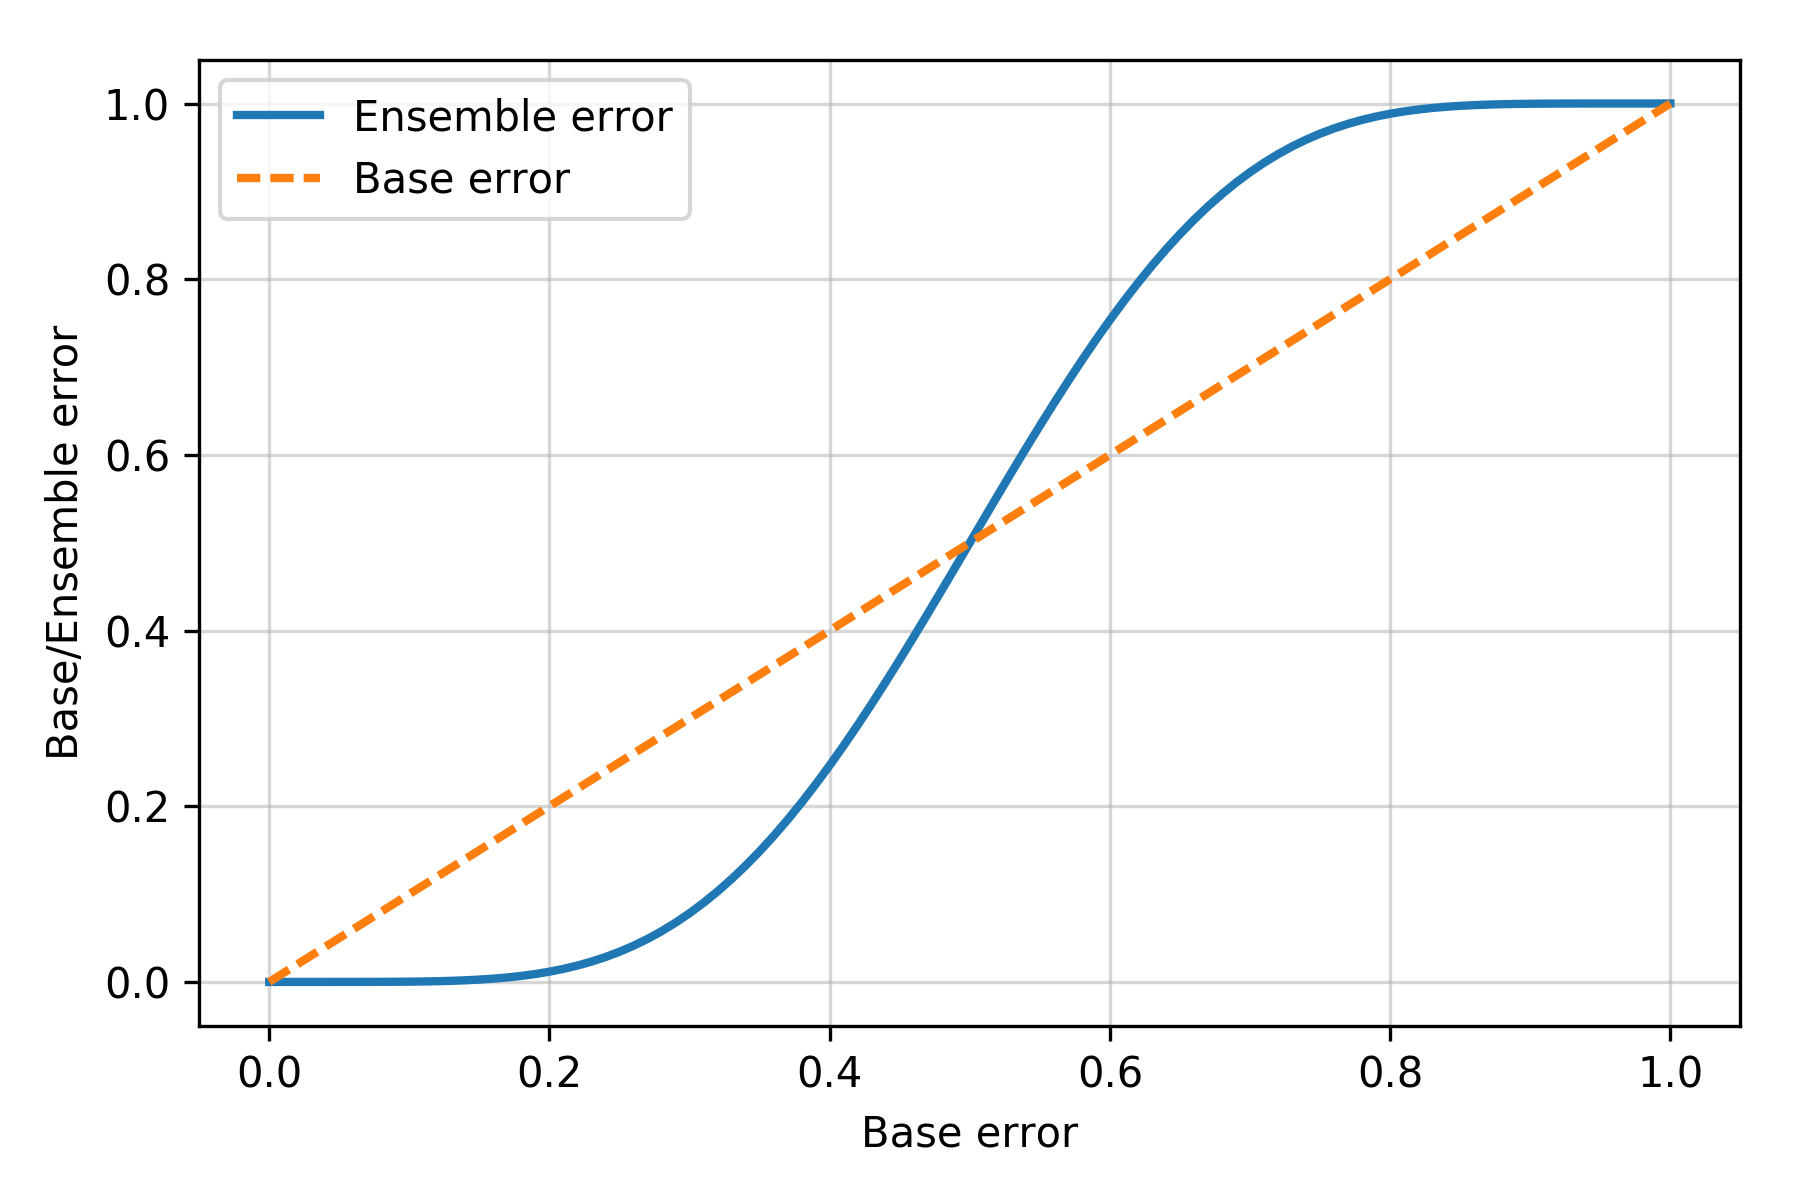
\includegraphics[scale=0.6]{Code/ch07/images/07_03.png}
\end{frame}

\begin{frame}
  \frametitle{Voting classifier in scikit-learn}
  \begin{itemize}
  \item Simply instantiate several classifiers
  \item Make a list
  \item Pass to sklearn.ensemble.VotingClassifier(...)
  \item  \href{http://scikit-learn.org/stable/modules/generated/sklearn.ensemble.VotingClassifier.html}{\beamergotobutton{API link}}
  \end{itemize}
\end{frame}

\begin{frame}[fragile]
\small
\begin{verbatim}
  clf1 = LogisticRegression(random_state=1)
  clf2 = RandomForestClassifier(random_state=1)
  clf3 = GaussianNB()
  estimators=[('lr', clf1), ('rf', clf2), ('gnb', clf3)]
  ens_clf = VotingClassifier(estimators)
  ens_clf = eclf1.fit(X, y)
\end{verbatim}
\end{frame}

\begin{frame}
  \frametitle{Boostrap aggregation (bagging)}
  \begin{itemize}
  \item We used the entire training set for the majority vote classifier
  \item Here we draw \textbf{bootstrap samples}
  \item In statistics, \textbf{bootstrapping} is any test or metric that relies on \textbf{random sampling with replacement}.
  \item Hypothesis testing: bootstrapping often used as an alternative to statistical inference based on the assumption of a parametric model when that assumption is in doubt
  \item The basic idea of bootstrapping is that inference about a population from sample data, can be modelled by resampling with replacement the sample data and performing inference about a sample from resampled data.
  \end{itemize}
\end{frame}

\begin{frame}
  \frametitle{Bagging}
  \center
  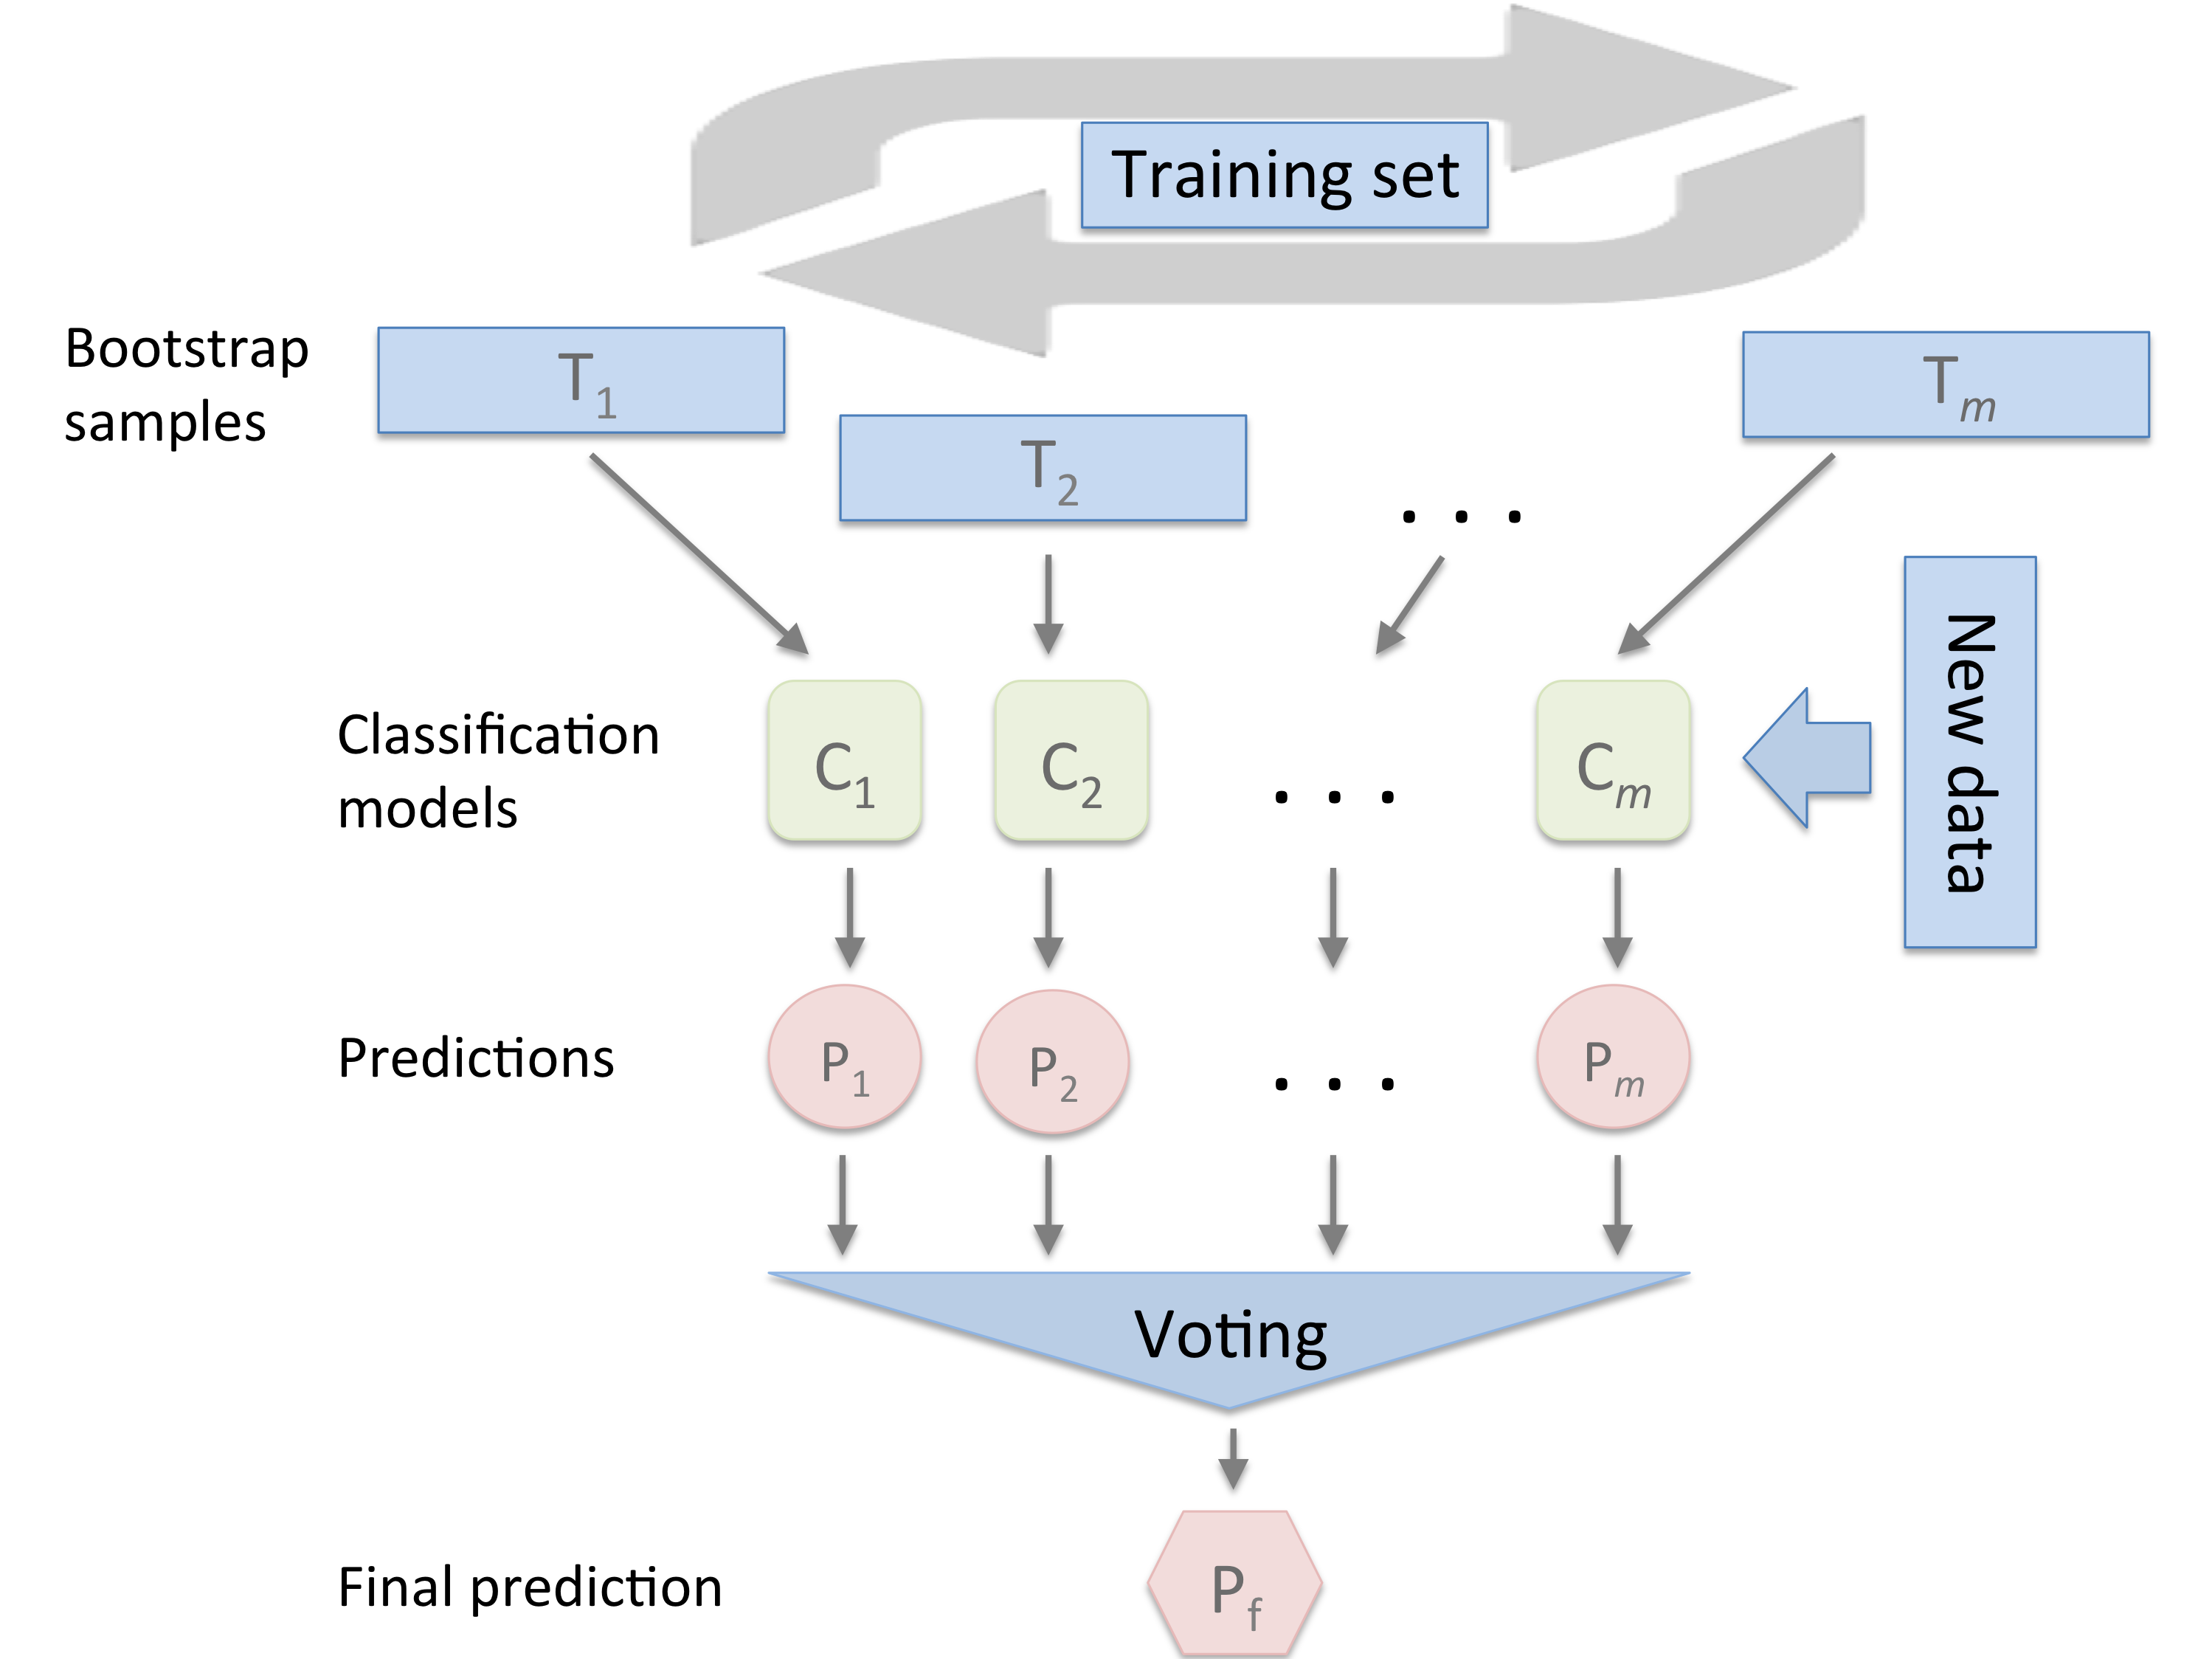
\includegraphics[scale=0.08]{Code/ch07/images/07_06.png}
\end{frame}

\begin{frame}
  \frametitle{Boostrapping example}
  \center
  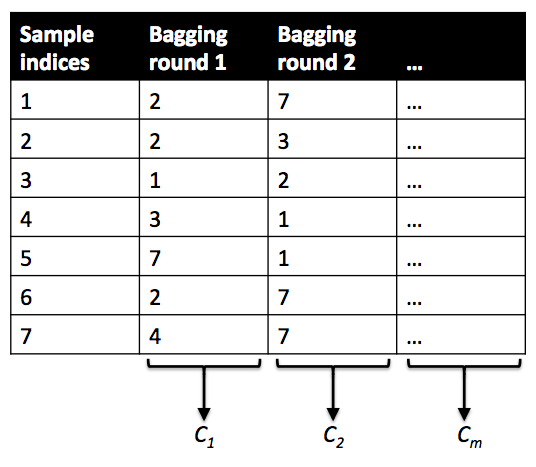
\includegraphics[scale=0.24]{Code/ch07/images/07_07.png}
  \begin{itemize}
  \item Seven training examples
  \item Sample randomly with replacement
  \item Use each boostrap sample to train a classifier $C_j$
  \item $C_j$ is typically a decision tree
  \item \textbf{Random Forests}: also use random feature subsets
  \end{itemize}

\end{frame}

\begin{frame}
  \frametitle{Bagging in scikit-learn}
  \begin{itemize}
  \item Instantiate a decision tree classifier
  \item Make a bagging classifier with decision trees
  \item Check that the accuracy is higher for the bagging classifier
  \item \href{https://github.com/rasbt/python-machine-learning-book/blob/master/code/ch07/ch07.ipynb}{\beamergotobutton{PML github}}
  \end{itemize}
\end{frame}

\begin{frame}
  \frametitle{Boosting}
  \begin{itemize}
  \item Basic idea: start with weak learners that have only a slight performance advantage over random guessing (e.g. a decision tree stump) and try to boost their performance by focusing on training samples that are hard to classify
  \item Very simple base classifiers learn from misclassified training examples
  \item The original boosting algorithm was formulated by Robert Schapire in 1990
  \item It was later refined into \textbf{AdaBoost}
  \item \textbf{AdaBoost} (short for Adaptive Boosting) is the most common implementation of boosting
  \end{itemize}
\end{frame}

\begin{frame}
  \frametitle{Original boosting algorithm}
  \begin{enumerate}
  \item Draw a random subset of training samples $d_1$ without replacement from the training set $D$ to train a weak learner $C_1$
  \item Draw second random training subset $d_2$ without replacement from the training set and add 50 percent of the samples that were previously misclassified to train a weak learner $C_2$
  \item Find the training samples $d_3$ in the training set $D$ on which $C_1$ and $C_2$ disagree to train a third weak learner $C_3$
  \item Combine the weak learners $C_1, C_2$, and $C_3$ via majority voting
  \end{enumerate}
\end{frame}

\begin{frame}
  \frametitle{AdaBoost}
  \begin{itemize}
  \item In contrast, AdaBoost uses the complete training set to train the weak learners
  \item Training samples are reweighted in each iteration to build a strong classifier
  \item End goal is to build a strong classifier that learns from the mistakes of the previous weak learners in the ensemble
  \end{itemize}
\end{frame}

\begin{frame}
  \frametitle{AdaBoost algorithm}
  \begin{enumerate}
  \item Set weight vector $\mathbf{w}$ to uniform weights where $\sum_i  w_i = 1$.
  \item For $j$ in $m$ boosting rounds, do the following:
  \begin{enumerate}
  \item Train a weighted weak learner: $C_j = train(\mathbf{X, y, w})$.
  \item Predict class labels: $\hat{y} = predict(C_j, \mathbf{X})$.
  \item Compute the weighted error rate: $\epsilon = \mathbf{w} \cdot (\mathbf{\hat{y}} \neq \mathbf{y})$.
  \item Compute the coefficient $\alpha_j$: $\alpha_j=0.5 \log \frac{1 - \epsilon}{\epsilon}$.
  \item Update the weights: $\mathbf{w} := \mathbf{w} \times \exp \big( -\alpha_j \times \mathbf{\hat{y}} \times \mathbf{y} \big)$.
  \item Normalize weights to sum to 1: $\mathbf{w}:= \mathbf{w} / \sum_i w_i$.
  \end{enumerate}
  \item Compute the final prediction: $\mathbf{\hat{y}} = \big( \sum^{m}_{j=1} \big( \mathbf{\alpha}_j \times predict(C_j, \mathbf{X})  \big) > 0 \big)$.
  \end{enumerate}
  \scriptsize
  \\~\\
  Notes: For clarity, we will denote element-wise multiplication by the cross symbol $(\times)$ and the dot product between two vectors by a dot symbol $(\cdot)$, respectively. Note that the expression ($\mathbf{\hat{y}} == \mathbf{y}$) in step 5 refers to a vector of 1s and 0s, where a 1 is assigned if the prediction is incorrect and 0 is assigned otherwise.
\end{frame}

\begin{frame}
  \frametitle{}
  \begin{itemize}
  \item
  \end{itemize}
\end{frame}

\end{document}
